\documentclass{article}
\usepackage{graphicx}
\usepackage{float}
\usepackage{amsfonts}
\usepackage{amsmath}
\usepackage{subfigure} 
\usepackage[ruled,vlined]{algorithm2e}
\usepackage{geometry}
\geometry{a4paper,scale=0.8}
\usepackage{listings}
\usepackage{color}

\definecolor{dkgreen}{rgb}{0,0.6,0}
\definecolor{gray}{rgb}{0.5,0.5,0.5}
\definecolor{mauve}{rgb}{0.58,0,0.82}


\lstset{
    %backgroundcolor=\color{red!50!green!50!blue!50},%代码块背景色为浅灰色
    rulesepcolor= \color{gray}, %代码块边框颜色
    breaklines=true,  %代码过长则换行
    numbers=left, %行号在左侧显示
    numberstyle= \small,%行号字体
    %keywordstyle= \color{blue},%关键字颜色
    commentstyle=\color{gray}, %注释颜色
    frame=shadowbox%用方框框住代码块
    }
\bibliographystyle{ieeetr}
\title{Summer Research Report}
\author{ZHANG HUAKANG}
\begin{document}
    \maketitle
    \section{Introduction}
        \subsection{Background}
            \paragraph{}
            The concept of cloud computing was first proposed in 2005 \cite{armbrust2010view} which means that the processing of big data is transferred to the server in the data center.. In 2006, Amazon's IaaS platform AWS was launched. Since then, cloud computing has profoundly changed human life. Internet of Things (IoT) was first proposed in 1999 \cite{iot}. With the development of IoT, large amounts of data are collected, uploaded and processed in the data center. In recent years, deep learning as a part of a broader family of machine learning methods based on artificial neural networks with representation learning is growing rapidly and is widely used in areas such as computer vision and natural language processing. Combined with IoT, it has given rise to many applications that have changed people's lives such as autonomous vehicle. But, due to the network bandwidth limitations and latency, centralized cloud computing architecture becomes inefficient and the computational task of deep learning is shifting from central servers to edge nodes gradually which is called edge computing. 
            \paragraph{}
            Edge nodes do not have high computing power due to manufacturing cost, size and other reasons, while reducing network bandwidth consumption and latency caused by communication with data center. How to reasonably allocate computing resources for multiple tasks on an edge node or cluster of edge nodes is critical to the improvement of edge computing efficiency.
    \section{Background}
        \subsection{Linux Container}
            \paragraph{}
            Compared with the traditional virtualization technology through hardware virtualization to create a software system independent of the host, Linux Container that share the same operating system kernel and isolate the application processes from the rest of the system will save a lot of computing resources for hypervisor to emulate hardware and improve efficiency (Figure \ref{img1} \cite{redhat}). In 2008, Docker came onto the scene with some new concept and technology. For example, Layers and Image version control enables developers to quickly build and deploy applications. Compared with the creation of a virtual machine that takes minutes or even hours, the creation of a new container can be completed in a few seconds.
            \begin{figure}[H]
                \centering
                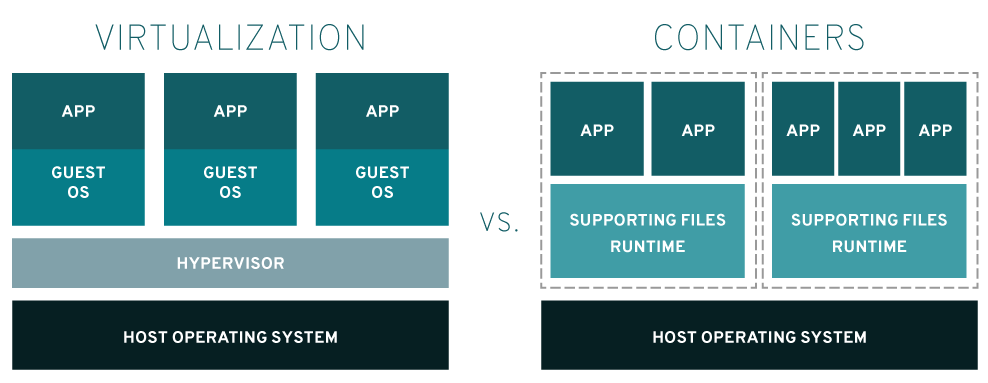
\includegraphics[width=.7\textwidth]{img/report1.png}
                \caption{Virtualization vs. Containers}
                \label{img1} 
            \end{figure}
        \subsection{GPU and GPU Virtualization}
            \paragraph{}
            CPU and GPU play completely different roles in computers. The CPU has  larger caches and a more powerful arithmetic logic unit(ALU), which allows the cpu to complete complex calculations in a short time, but the parallel computing performance is not high. The GPU has smaller caches and a large number of ALU, which makes the GPU have higher performance in performing parallel computing. In other words, GPU is more suitable for performing compute-intensive tasks, such as deep learning.
            \paragraph{}
            Therefore, how to allocate GPU computing resources is particularly important when processing multiple deep learning tasks. Nvidia launched GRID K1 in 2013, marking the maturity of GPU virtualization technology \cite{herrera2014nvidia}. After nearly a decade of technological development, there are many complete solutions in the cloud computing field such as Ailiyun's cGPU, Tencent's GaiaGPU\cite{8672318} and Nvidia's Volta MPS\cite{nvidiamps}. But all of them  focus on GPU virtualization in the cloud computing field instead of edge computing. For example, cGPU is only used for Alibaba Cloud's GPU server.
    \section{Design and Implementation}
        \subsection{Design}
            \subsubsection{Capture Video by Camera}
                \paragraph{}
                Cameras on nodes like Jetson Nano and Raspberry Pi will will record video for a given period of time, such as 10 seconds and save those video. The set of all videos from the same camera $Cam_i$ are called Task $T _i$, i.e. $T_i=\{V_{i,1},V_{i,2},V_{i,3}...V_{i,m}\}$. When a new video $V_{i,m}$ from $Cam_i$ is generated, the information about this video will be added to the Video Queue $Q_i$ (Figure \ref{img2}).
                \begin{figure}[H]
                    \centering
                    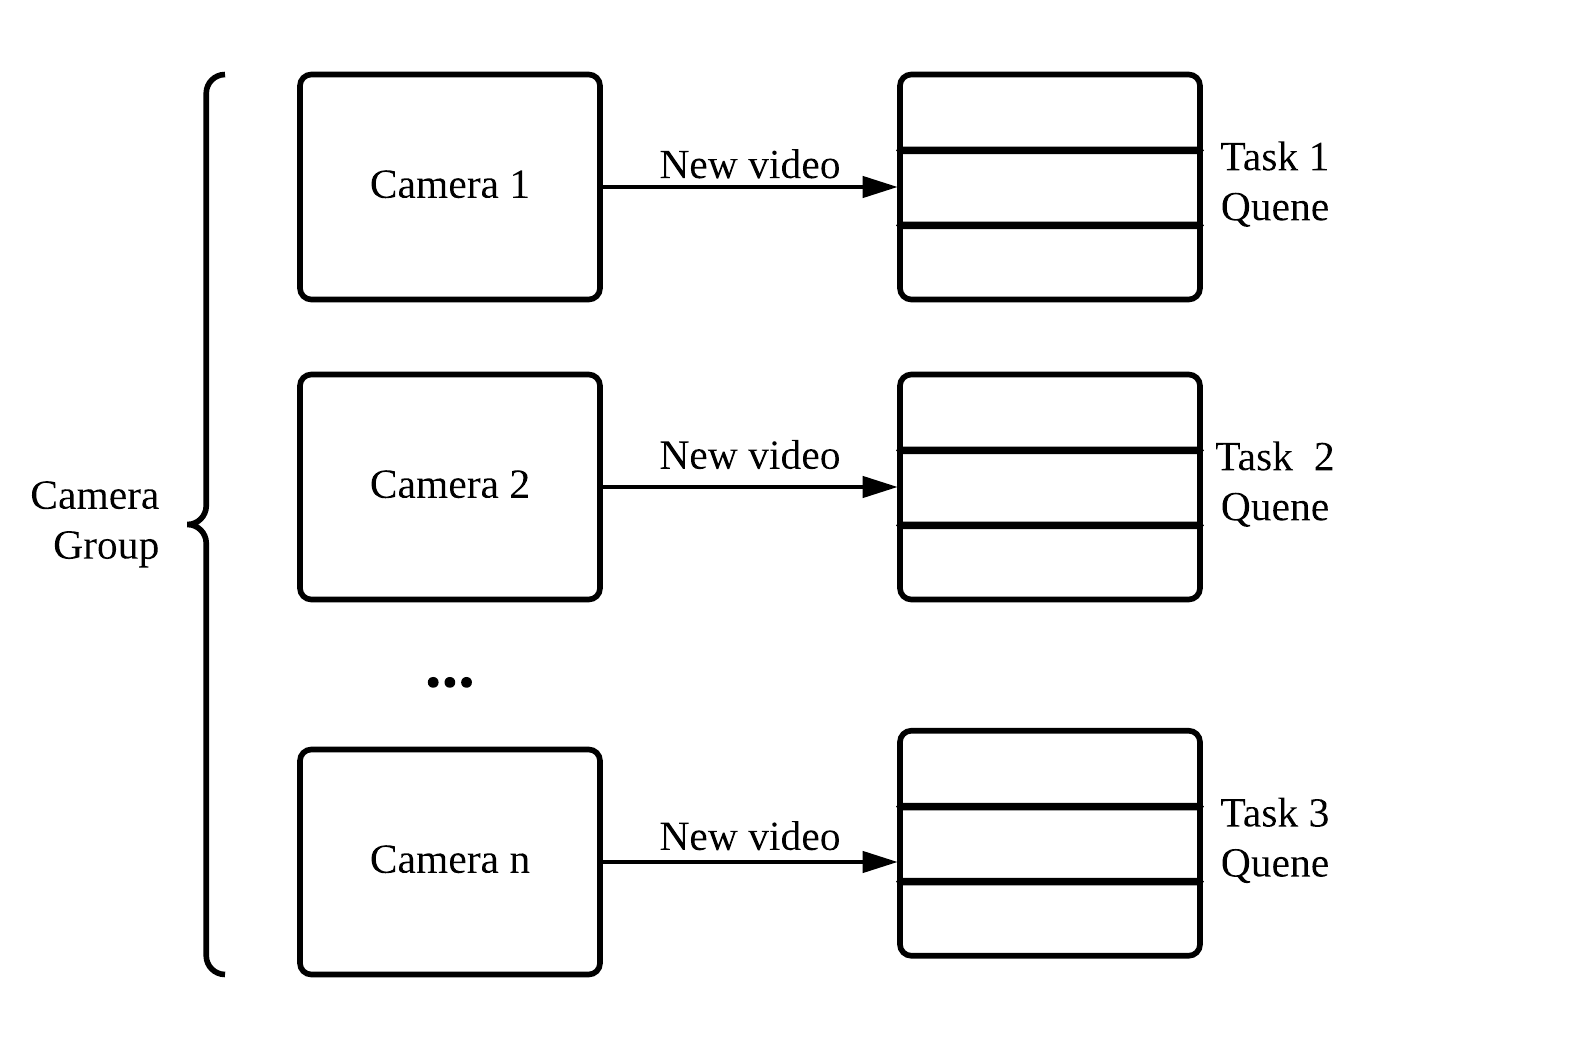
\includegraphics[width=0.8\textwidth]{img/report2.png}
                    \caption{Cameras capture and save video}
                    \label{img2} 
                \end{figure}
            \subsubsection{Assign Task to Container}
                \paragraph{}
                The video $V_{i,top}$ at the top of each Video Quene $Q_i$ will be put into the Task Set in manage program representing the task $T_i$ needs to be processed if the cardinality $|Q_i|>0$.  If the container $Con_f$ in Containers Set $\{Con_1,Con_2,...,Con_m\}$ is free, the video $V_{j,top}$ will be assign to this container.  
                \paragraph{}
                In a container, when a new video is assigned, the program in the container will start to run and generate output files, which can be statistical results and rendering files for target detection. The output $O_{j,top}^f$ will be return to the manage program as the e basis to make the next allocation (Figure \ref{img3}).
                \begin{figure}[H]
                    \centering
                    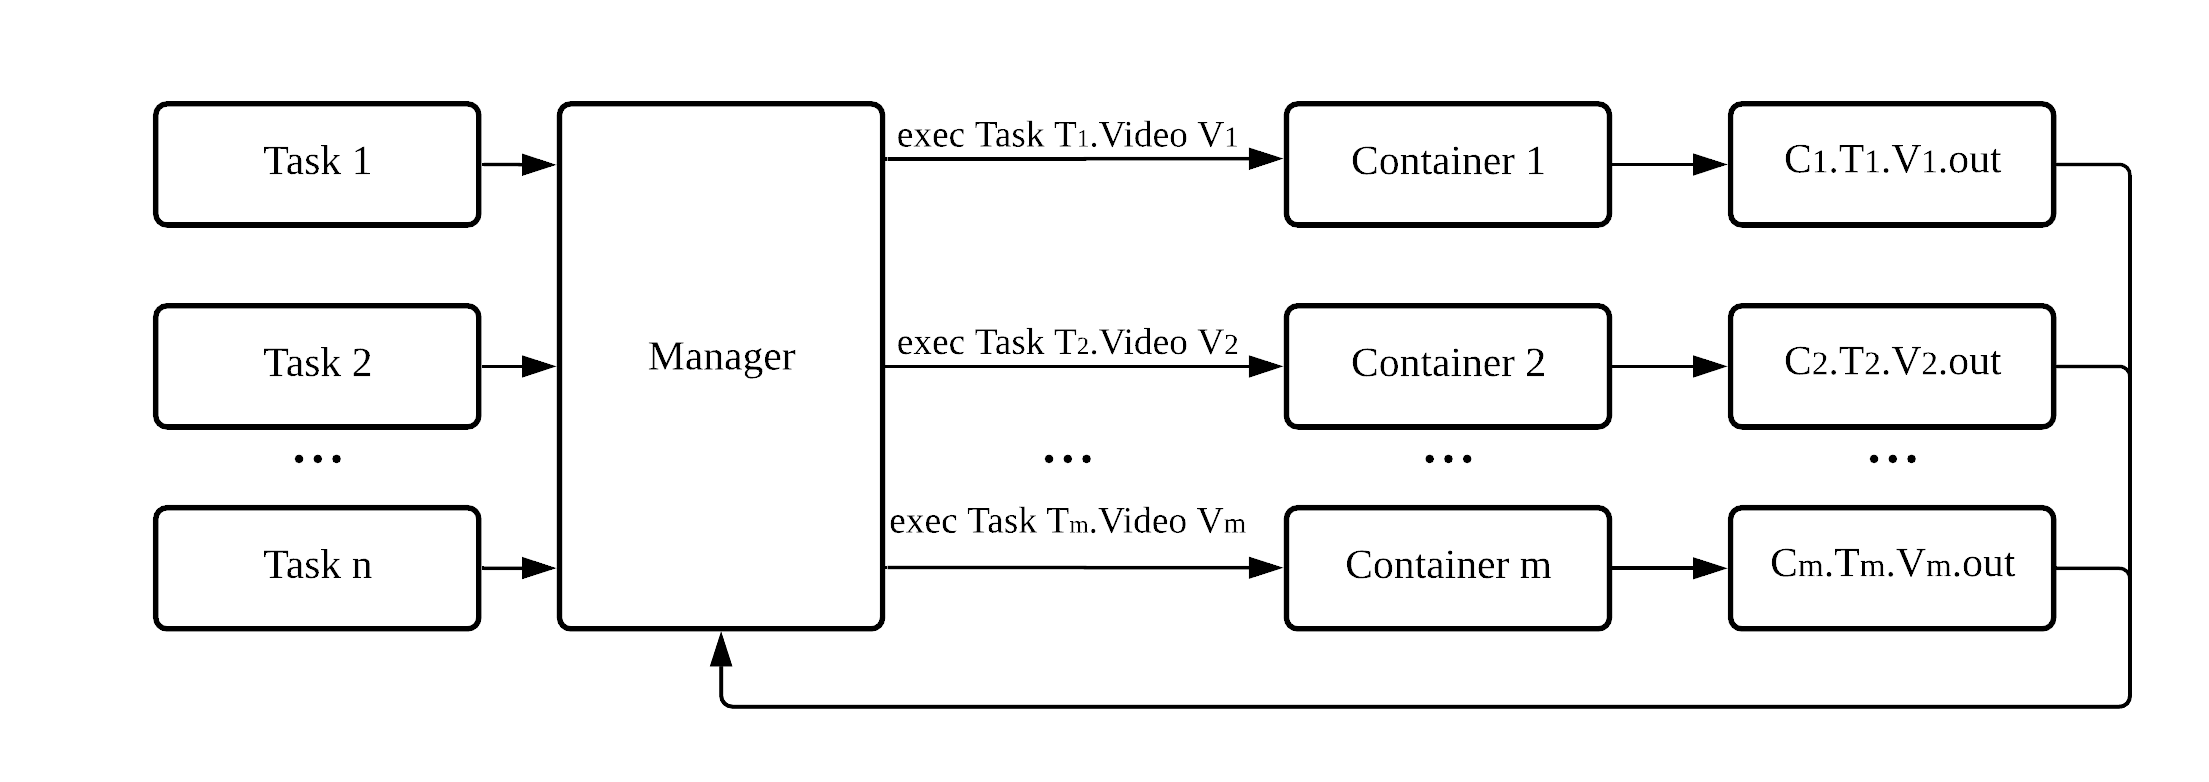
\includegraphics[width=01\textwidth]{img/report3.png}
                    \caption{Assign Task to Container}
                    \label{img3} 
                \end{figure}
                \paragraph{Update Weights}
                Here is a simple algorithm to update task's weights. Assume that the output $O_{j,top}^f$ of the program in container $Con_f$ is the number of times an object has been detected. We know the total number of object in each task $T_i$ is $Total_{obj,i}$ and a factor $k\in \mathbb{R}^+$. The new weight of task $T_j$

                $$Total_{obj,j}^{'}=k\times Total_{obj,j}+O_{j,top}^f$$
                $$Total_{obj}^{'}=\sum_{T_i\neq T_j} Total_{obj,i}+Total_{obj,j}^{'}$$
                $$w_j=\frac{Total_{obj,i}^{'}}{Total_{obj}^{'}}$$
                Factor $k$ represents the influence of the video at different times on the current weight.
                $$Total_{obj,i}=O_{j,top}+kO_{j,top-1}+k^2O_{j,top-2}+...+k^{top}O_{j,0}$$ 
                $k\in (0,1)$ means that the closer the video time to the current video time, the greater the influence on the current weight. $k=1$ means all videos are equal. And $k>1$ means that the closer the video time to the current video time, the smaller the influence on the current weight.

                % \begin{algorithm}[H]
                %     \SetAlgoLined
                %     \KwData{total number of target object in all task $Total_{obj}$, total number of target object in task $T_j$ $Total_{obj,j}$ and the factor $k$}
                %     \KwIn{the output $O_{j,top}^k$}
                %     \KwOut{the new weight $w_j$ of task $T_j$}
                %     $Total_{obj}$ = $Total_{obj}-Total_{obj,i}$\;
                %     $Total_{obj,i}$ = $k\times Total_{obj,j}+O_{j,top}^k$\;
                %     $Total_{obj}$ = $Total_{obj}+Total_{obj,i}$\;
                %     $w_j=Total_{obj,j}/Total_{obj}$
                %     \caption{Update Task Weight}
                % \end{algorithm}
                \paragraph{}
                It can be prove that
                \begin{equation}
                    \begin{split}
                        \sum_{T_i}w_i=&\frac{\sum_{T_i\neq T_j}Total_{obj,i}+Total_{obj,j}^{'}}{Total_{obj}^{'}}\\
                            =&1
                    \end{split}
                \end{equation}
                \paragraph{}
                After updating the weight, the manage program will check the Task Set and find a Task $T_k$ whose proportion of the container is less than its weight $w_i$, assign it to the free container $Con_f$.

                \begin{algorithm}[H]
                    \SetAlgoLined
                    \KwData{total number of conatiners $N_{Con}$, number of containers that currently executing task $T_i$ $N_{Con_i}$}
                    \While{Task Set is not empty}{
                        \If{new output $O_{j,top}^k$ is generated}{
                            the weight $w_j$ = updateWeight($O_{j,top}^k$)\;
                            \ForEach{video $V_{i,top} \in $Task Set}{
                                \If{$N_{Con_i}/N_{Con}<w_i$ and $|Q_i|\neq 0$ }{
                                    % \tcp{$|Q_i|=0$ if all videos of this task  has been processed } 
                                    assignTask($V_{i,top}$ , $Con_i$)\;
                                    break\;
                                }
                            }
                        }
                    }
                    \caption{Assigning tasks to containers}
                \end{algorithm}

            \subsubsection{Example}
                \paragraph{}
                Here we have $2$ cameras(tasks) recording the videos, i.e. $Task_1$ and $Task_2$, and four container $Con_1,Con_2,Con_3,Con_4$. At first, two of them have same weight $0.5$, thus each task has two containers processing. When all four containers finish processing the third video, the weights of the two tasks change from $\{0.5,0.5\}$ to $\{0.75,0.25\}$. When the next task is assigned, one of the containers of $T_2$ will execute $T_1$ (Figure \ref{img4}).
            \begin{figure}[H]
                \centering
                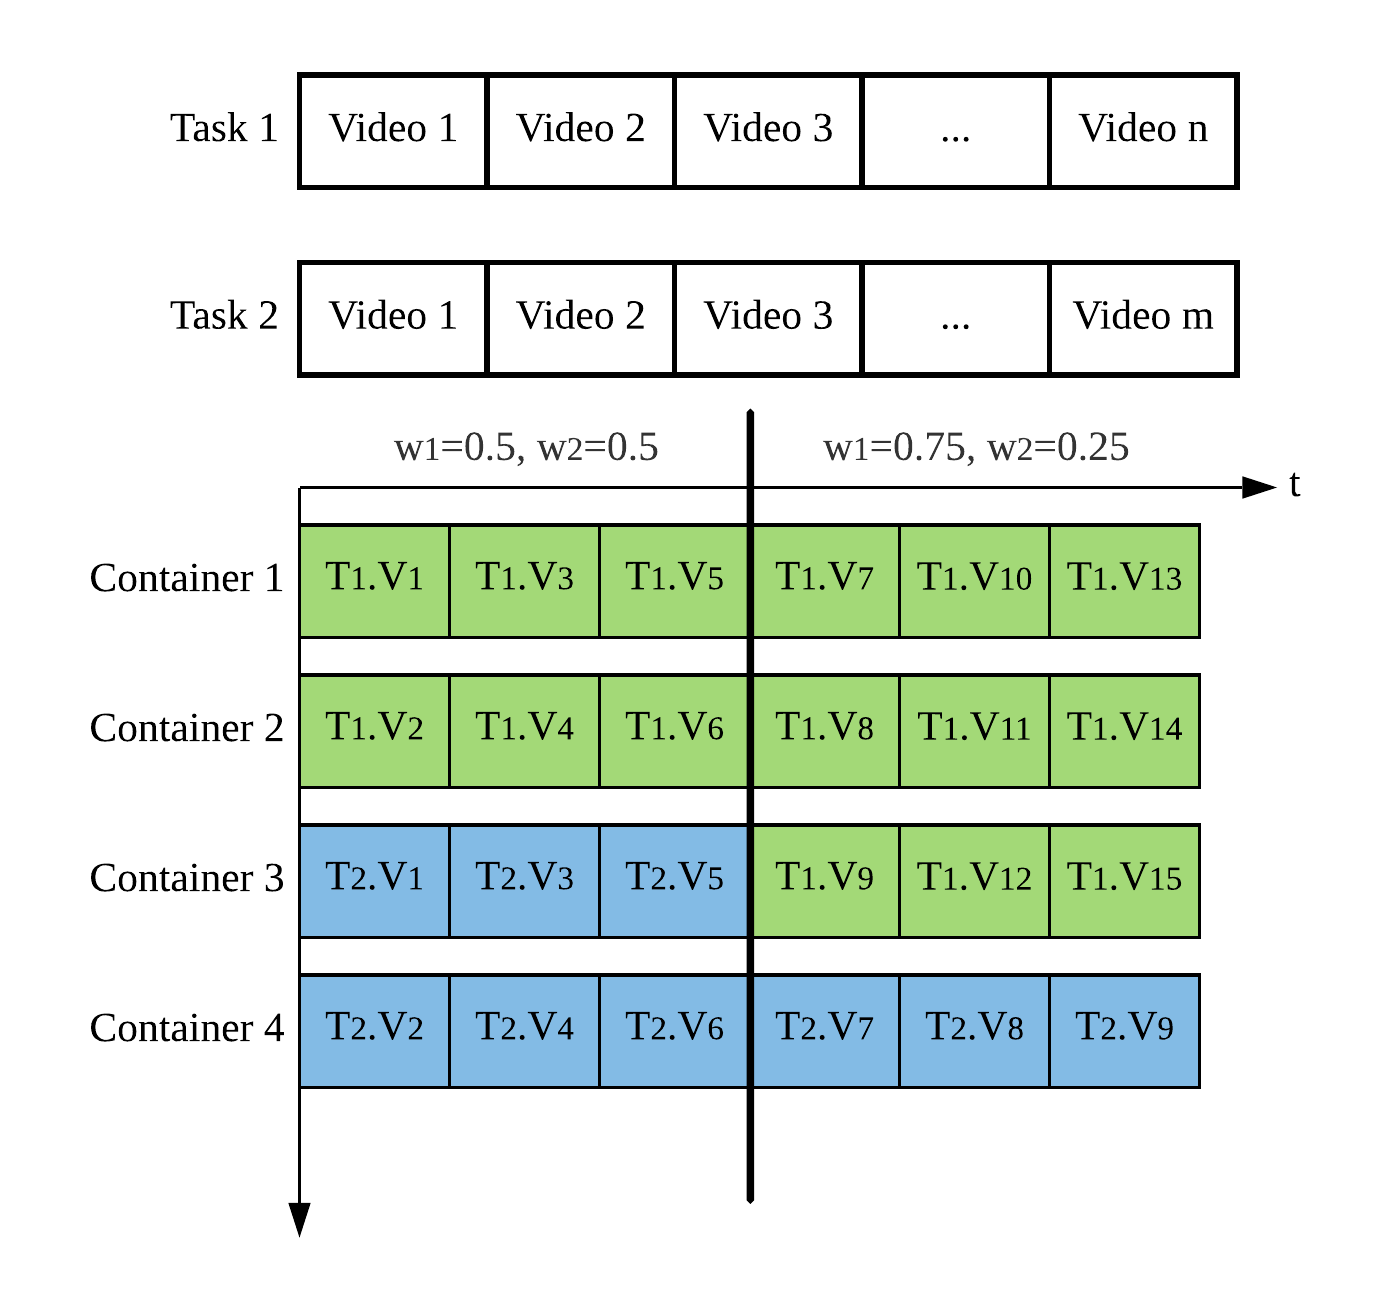
\includegraphics[width=.8\textwidth]{img/report4.png}
                \caption{Example}
                \label{img4} 
            \end{figure}
        \newpage
        \subsection{Implementation}
            \subsubsection{Docker Image Build}
                    \begin{lstlisting}
FROM python
RUN mkdir /code
COPY test.py /code
COPY requirements.txt /code
WORKDIR /code
RUN pip3 install -r requirements.txt
WORKDIR /code
CMD ["python3","/code/test.py"]
                    \end{lstlisting}
            \subsubsection{Check output}
                    \begin{lstlisting}
import os
class Manager:              
    def checkOutput(self):
        BASE_DIR = os.path.dirname(os.path.abspath(__file__))
        outputPath=os.path.join(BASE_DIR, 'output')
        fileList=os.listdir(outputPath)
        fileList = sorted(fileList, key=lambda x: os.path.getmtime(os.path.join(outputPath, x)))
        fileNumInLastUpdate= len(fileList)
        with True:
            fileList = sorted(fileList, key=lambda x: os.path.getmtime(os.path.join(outputPath, x)))
            if len(fileList)>fileNumInLastUpdate:
                fileNumInLastUpdate+=1
                with open(os.path.join(outputPath,fileList[len(fileList)-1]),'r') as f:
                    output=f.readline ()
                    curTaskNo=int(outputName.split('-')[0])
                    assignTask(fileList[len(fileList)-1],int(output),curTaskNo)
                    \end{lstlisting}
            \subsubsection{Update weights}
                \begin{lstlisting}
class Task:
    def __init__(self,path):
        self.path=path
        self.num=0
        self.conNum=0
        self.topVideo=None
class Manager:
    def __init__(self):
        self.k=1
        self.tasks=[Task('1'),Task('2')]
    def updateWeight(self,taskNo,output):
        self.tasks[taskNo].num=self.k*self.tasks[taskNo].num+output
    def getWeight(self,taskNo):
        sum=0
        for task in tasks:
            sum+=task.num
        return self.tasks[taskNo]/sum
                \end{lstlisting}
            \subsubsection{Assign task}
                \begin{lstlisting}
import os
class Container:
    def __init__(self,cpuShares,folderPath,image):
        self.id=os.system("docker run -d --cpus={} --runtime nvidia -v  {}:/code {} {}".format(cpuShares,folderPath,image))   
    def execTask(tak):
        BASE_DIR = os.path.dirname(os.path.abspath(__file__))
        inputPath=os.path.join(BASE_DIR, 'input')
        inputFile=os.path.join(inputPath,self.id)
        f = open(inputFile,w) 
        f.wirte(task.topVideo)
        f.close

class Manager:
    def __init__(self,folderPath,image):
        self.containers=[]
        for i in range(2):
            self.containers.append(Container(getWeight(i),folderPath),image)
    def assignTask(outputName,output, curTaskNum):
        self.tasks[curTaskNum].conNum-=1
        curCon=outputName.split('-')[1]
        for n in range(len(self.tasks)):
            if self.tasks[n].conNum/len(self.containers)<self.getWeight(n):
                self.tasks[n].conNum+=1
                self.containers[curCon].execTask(self.tasks[n])
                break
                \end{lstlisting}
    \newpage
    \section{Demo}
        \paragraph{}
        In Figure \ref{img5}, the first image shows that the output of the program in conatiner when starting. In addition, 'detach' mode is also availiable. The second image is an time usage result of a frame. \textit{CPU} is the time CPU uses. \textit{CUDA} is the the time the GPU uses. \textit{Pre-Process} is mainly file IO such as getting the image from the video.  The longest time is used by the \textit{Network} part which uses model to process image. \textit{Post-Process} and \textit{Visualize} are about some computation after the Network computation like counting time-consuming, and rendering result. Figure \ref{img7} are four outputs of vehicle recognition. 
        \begin{figure}[H]
            \centering
            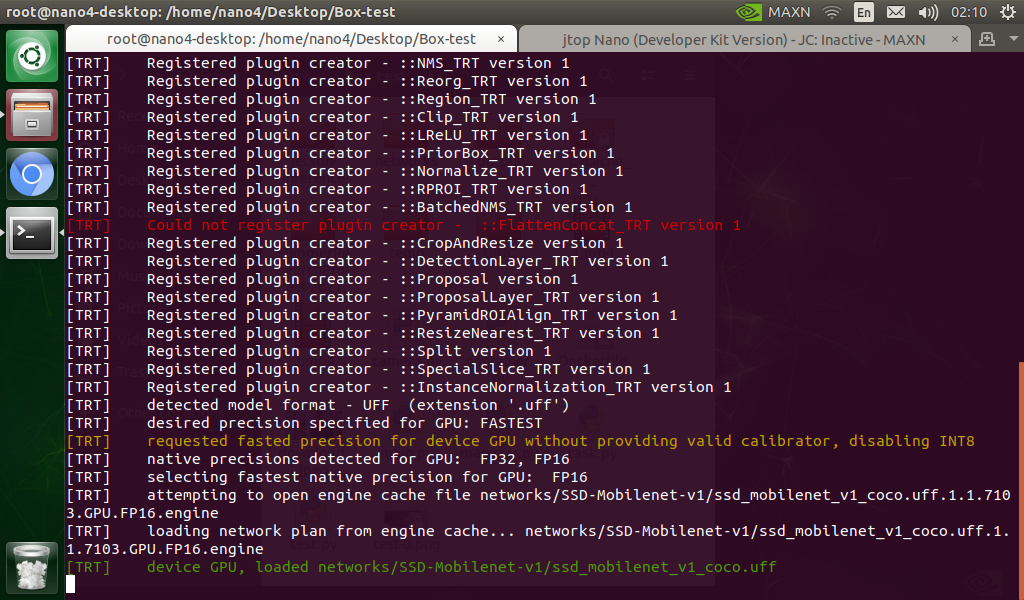
\includegraphics[width=.6\textwidth]{img/report11.png}
            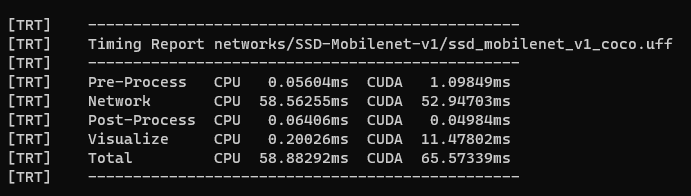
\includegraphics[width=.6\textwidth]{img/report6.png}
            \caption{Demo}
            \label{img5}
        \end{figure}
        \begin{figure}[H]
            \centering
            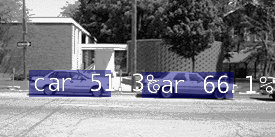
\includegraphics[width=.4\textwidth]{img/output1.jpg}
            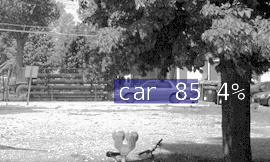
\includegraphics[width=.4\textwidth]{img/output2.jpg}
            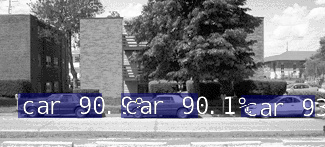
\includegraphics[width=.4\textwidth]{img/output3.jpg}
            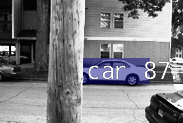
\includegraphics[width=.4\textwidth]{img/output4.jpg}
            \caption{Output}
            \label{img7}
        \end{figure}
        Figure \ref{img6} shows the resource monitoring interface. The first image on the first line is the overview. The second image is the GPU usage by time without executing any task. The first image in the second line is quad-core CPU usage. The second image is the GPU usage when there are task in progress.
        \begin{figure}[H]
            \centering
            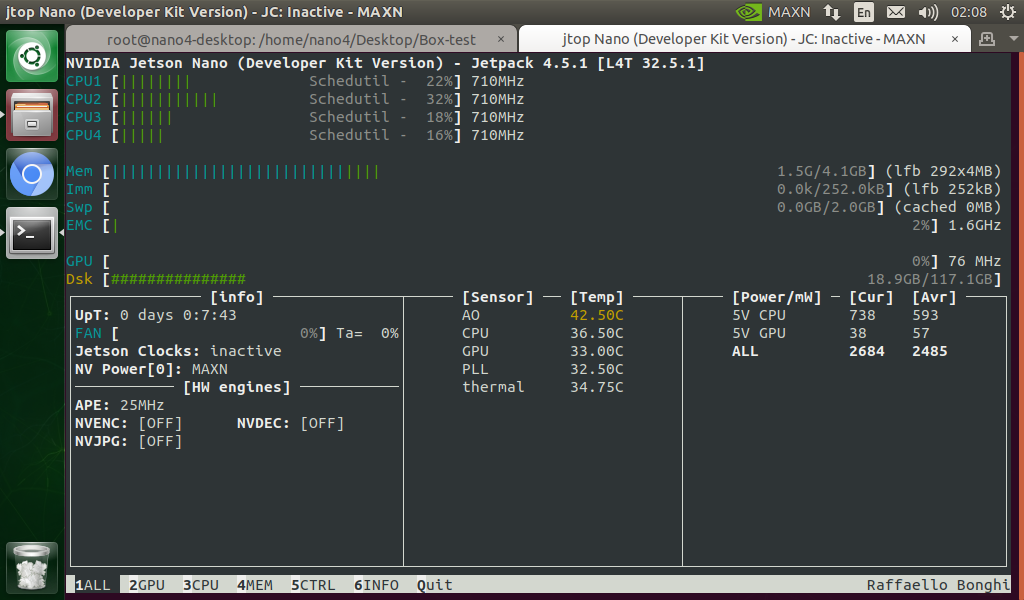
\includegraphics[width=.4\textwidth]{img/report7.png}
            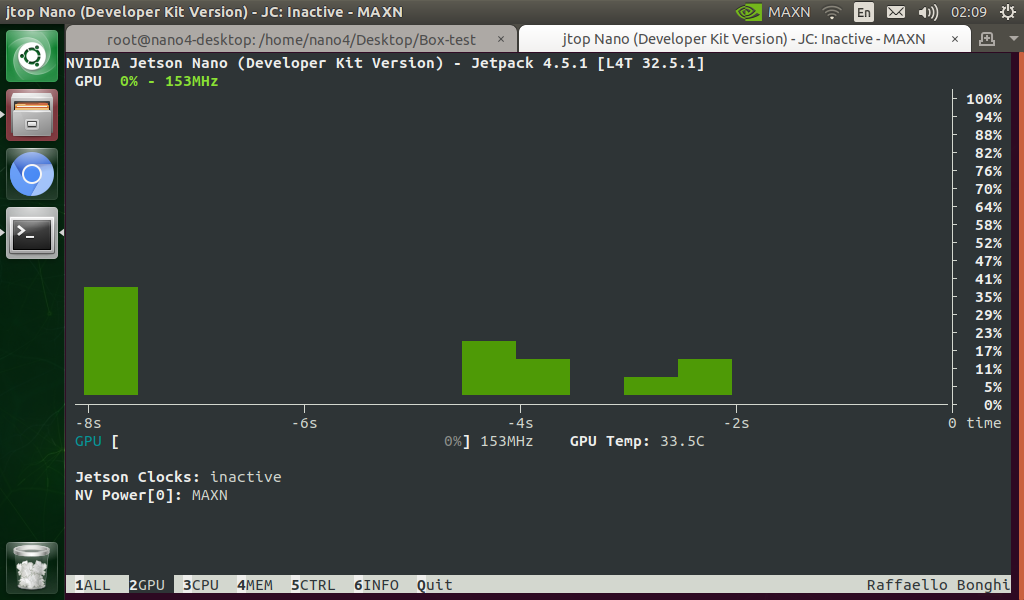
\includegraphics[width=.4\textwidth]{img/report8.png}
            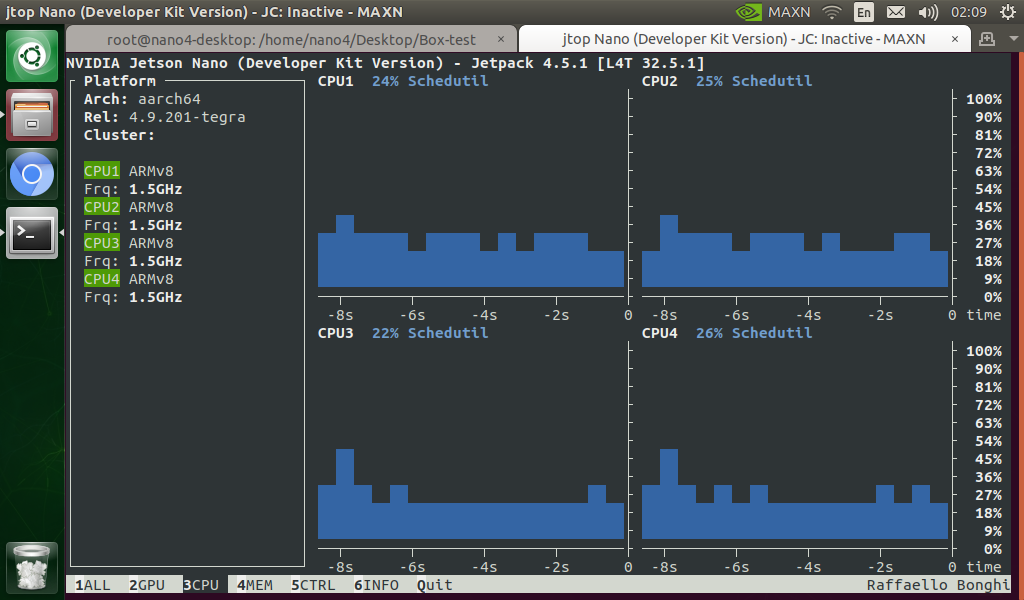
\includegraphics[width=.4\textwidth]{img/report9.png}
            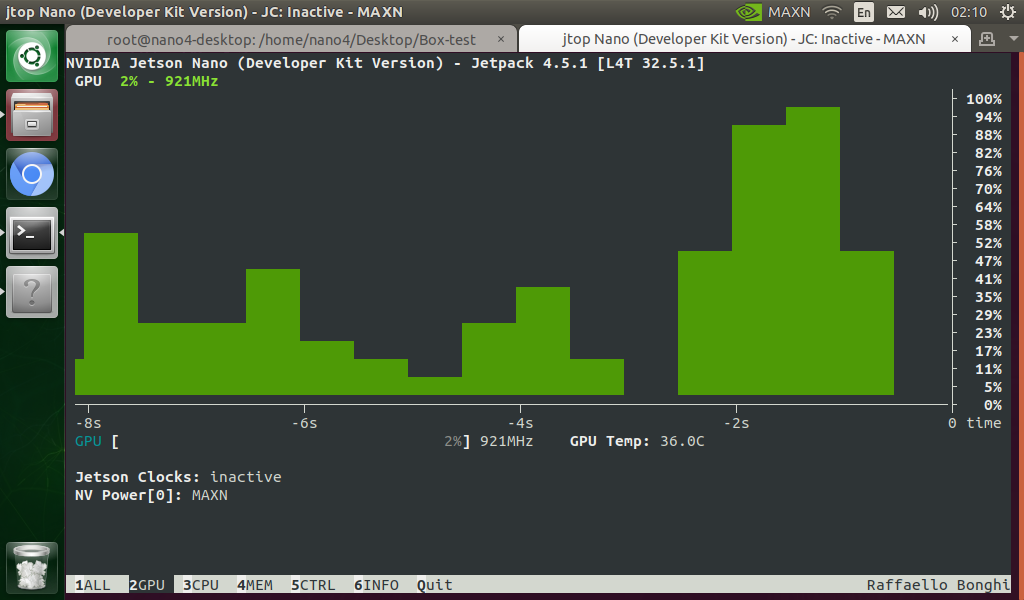
\includegraphics[width=.4\textwidth]{img/report10.png}
            \caption{Resources Usage}
            \label{img6}
        \end{figure}
    \section{Conclusion}
        \paragraph{}
        In this report, I propose a implementation of computing power allocation. This method is different from the traditional GPU virtualization method by simulating the hardware. By dividing the task into blocks, multiple containers can execute the same task to implement the allocation of different computing power to different tasks. But due to the limitations of the Docker Engine, the smallest allocation unit is a entire card.
    \bibliography{reportref}
\end{document}